%!TEX root = origin_elements_lecture_notes.tex

\chapter{Slow Neutron Capture Nucleosynthesis}\label{ch:s-process}

We have seen that fusion is energetically favorable up to the iron peak, with \ex{62}Ni having the highest binding energy of $8.7945$\,MeV per nucleon. Furthermore, the Coulomb energy -- see equation~\eqref{eqn:massive_stars:coulomb_energy} -- is too high even during silicon burning already in order to directly combine two nuclides. Charged particle reactions are thus highly unlikely to contribute to nucleosynthesis beyond the iron peak. Neutrons on the other hand are uncharged, thus can pass through the Coulomb barrier without any issues and induce nuclear reactions. In this chapter we will first look at slow neutron capture reactions, observations and astrophysical sites, and finally briefly discuss the modeling of these reactions.


\section{Neutron Captures} \label{sec:s-process:neutron_captures}

In the \acf{sproc}, the probability of capturing more than one neutron is generally lower than the probability that a nucleus, if unstable, decays via $\beta^-$-decay. The \ac{sproc} thus follows in the chart of the nuclides along the valley of stability. 
\begin{figure}[tb]
    \centering
    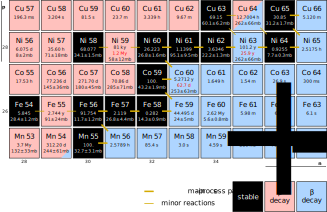
\includegraphics[width=0.9\textwidth]{graphics/s-process/feni_chartnuc}
    \caption{The \ac{sproc} around the iron peak. Due to its high abundance, \ex{56}Fe is the main seed from which the \ac{sproc} starts.}
    \label{fig:s-process:feni_chartnuc}
\end{figure}
Figure~\ref{fig:s-process:feni_chartnuc} shows an excerpt of the chart of the nuclides focusing around the iron peak. Due to its high abundance, \ex{56}Fe is the main seed for the \ac{sproc}. The thick and thin arrows in Figure~\ref{fig:s-process:feni_chartnuc} show the main \ac{sproc} path and minor reaction paths, respectively. Also given are the Maxwellian-averaged nuclear cross sections from the KADoNiS database.\footnote{\url{https://kadonis.org}} These cross sections are printed in italic if they have only been determined theoretically. Finally, half-lives are given at laboratory conditions in black and at \ac{sproc} relevant stellar conditions in red, if different.

In Figure~\ref{fig:s-process:feni_chartnuc}, for example, most of the produced \ex{63}Ni nuclei will capture another neutron in order to form \ex{64}Ni since the half-life of \ex{63}Ni is, even under stellar conditions, long enough such that this nucleus is mostly stable with respect to the \ac{sproc}. However, branching points with shorter half-lives that can have important effects on \ac{sproc} nucleosynthesis exist.


\subsection{Nuclear Reaction Rates}

We have so far mostly looked at the so-called $Q$-value, i.e., the energy released in a give nuclear reaction, in order to determine the likelihood of a reaction to take place. Energy release is however not always the dominating factor. As an example, we have discussed photodisintegration reactions, e.g., during oxygen burning -- see reactions~\eqref{eqn:massive_stars:oxygen_burning_reactions} -- that take place in massive stars even though these reactions consume energy. In a stellar environment, two additional quantities influence how likely it is for a reaction to take place. These quantities are the nuclear cross section $\sigma$ and the velocity distribution of particles in the plasma. 

Nuclear cross sections generally depend on the relative velocities of projectiles and targets, thus we can write $\sigma = \sigma(v)$. Furthermore, if the velocities follow a distribution $P(v)$ with
\begin{equation}
    \int_0^\infty P(v) dv = 1,
\end{equation}
we can write
\begin{equation}
    \int_0^\infty v P(v) \sigma(v) dv = \langle \sigma v \rangle.
\end{equation}
Here, $\langle \sigma v \rangle$ contains all information on the nuclear physics. The reaction rate $r$ for two different particles to interact can then be written as
\begin{equation}
    r = N_a N_b \langle \sigma v \rangle_{ab},
\end{equation}
where $N_a$ and $N_b$ are the respective number densities of particles $a$ and $b$. If both particles are the same this reaction rate simplifies to
\begin{equation}
    r = \frac{N_a (N_a - 1)}{2}\langle\sigma v\rangle_{aa} \overset{N_a\gg1}{\approx} \frac{N_a^2}{2}\langle\sigma v \rangle_{aa}.
\end{equation}
Using the Kronecker symbol $\delta_{ab}$, we can write the overall reaction rate for an arbitrary velocity distribution as
\begin{equation}
    r_{ab} = \frac{N_a N_b \langle\sigma v\rangle_{ab}}{1 + \delta_{ab}}.
\end{equation}
% For practical reasons, the reaction rate in the literature is often reported as $N_A \langle\sigma v\rangle_{ab}$, where $N_A = 6.022 \times 10^{23}$\,mol$^{-1}$ is the Avogadro constant.

For non-relativistic and non-degenerate stellar plasmas, the velocities of particles will follow a Maxwell-Boltzmann distribution. Depending on the temperature, the Maxwell-Boltzmann velocity distribution has its maximum at
\begin{equation}
    v_T = \sqrt{\frac{2k_B T}{m_{ab}}}. \label{eqn:s-process:max_velocity_mb}
\end{equation}
Here, $k_B = 1.380 \times 10^{-23}$\,J\,K$^{-1}$ is the Boltzmann constant and
\begin{equation}
    m_{ab} = \frac{m_am_b}{(m_a + m_b)} \label{eqn:s-process:reduced_mass}
\end{equation} 
the reduced mass of the system. The reaction rate per particle pair can then be expressed as
\begin{equation}
     \langle \sigma v \rangle_{ab} = \left( \frac{8}{\pi m_{ab}} \right)^{\nicefrac{1}{2}} (kT)^{-\nicefrac{3}{2}} \int_0^\infty E\sigma(E) \exp\left(-\frac{E}{kT}\right)dE.
 \end{equation} 

 For neutron-induced reactions, which are the ones of importance in the \ac{sproc}, the reaction rate is generally expressed in terms of a \ac{macs} as
 \begin{equation}
     \langle\sigma\rangle_T = \frac{4}{\sqrt{\pi} v_T^2} \int_0^\infty v\sigma_n(v) \left(\frac{v}{v_T}\right)^2 \exp\left[-\left(\frac{v}{v_T}\right)^2\right]dv. \label{eqn:s-process:macs}
 \end{equation}

Databases such as KADoNiS\footnote{\url{https://kadonis.org}} are generally used to look up the best \ac{macs} for a given nucleus. The total \ac{macs} are typically given at a specific energy, in KADoNiS usually at 30\,keV, which is the energy relevant for the \ac{sproc}.


\subsection{Half-Lives}

Half-lives of nuclei that disintegrate via $\beta$-decay are not always the same under laboratory and stellar conditions. One example of this is bound-state $\beta$-decay. At high temperatures, e.g., temperatures that exist in stars, a certain nucleus might have so few electrons due to ionization that it becomes unstable. In this case it would decay via $\beta^-$-decay and thus transfer a neutron into a proton and an electron. Depending on the ionization level, the half-life drastically shortens compared to neutral atoms. One example of this is \ex{187}Re. Under laboratory conditions, \ex{187}Re has a half-life or around $4.3\times10^{10}$\,a. When fully stripped however, the half-life reduces to $<100$\,a \citep{nolden97}.

Under stellar conditions and thus for highly ionized atoms, calculations for the $\beta$-decay half-lives were done by \citet{takahashi87}. These authors present decay rates for various relevant temperatures and electron number densities.


\subsection{Capturing Neutrons Slowly}

Let us first look at the horizontal transitions of the \ac{sproc}, i.e., at transitions between stable nuclei. This formalism also applies to an unstable nucleus if the half-life is long compared to the probability of capturing another neutron. The rate of change of the number density of a stable nucleus with mass number $A$ can then be written as
\begin{equation}
    \frac{dN_A}{dt} = -N_n(t) N_A \langle\sigma v\rangle_A + N_n(t) N_{A-1} \langle\sigma v\rangle_{A-1}.
\end{equation}
Here, $N_n(t)$ is the number density of free neutrons, which may very with time. Since the reaction rate depends on the velocity, which itself is defined by the temperature of the environment, we can assume that $\langle\sigma v\rangle$ is constant if the temperature does not change. 

Replacing the reaction rate per particle with the \ac{macs}, see equation~\eqref{eqn:s-process:macs}, we can write $\langle \sigma v\rangle_{A} = \langle \sigma \rangle_{A} v_T$, and thus
\begin{equation}
    \frac{dN_A}{dt} = v_T N_n(t) \left[-N_A \langle\sigma\rangle_A + N_{A-1} \langle \sigma \rangle_{A-1} \right]. \label{eqn:s-process:dna_dt_intermediate_step}
\end{equation}

Since all isotopes experience the same neutron abundance, we can introduce the neutron exposure as
\begin{equation}
    \tau = v_T \int N_n(t)dt. \label{eqn:s-process:neutron_exposure}
\end{equation}
This can also be written as $d\tau = v_T N_n(t)dt$. We can now replace the time variable $t$ in equation~\eqref{eqn:s-process:dna_dt_intermediate_step} with the neutron exposure $\tau$ and thus get
\begin{equation}
    \frac{dN_A(\tau)}{d\tau} = -N_A(\tau)\langle\sigma\rangle_A + N_{A-1}(\tau)\langle\sigma\rangle_{A-1}. \label{eqn:s-process:dna_dtau}
\end{equation}


\subsection{Local Approximations}\label{sec:s-process:local_approximation}

For the \ac{sproc} we can determine the following boundary conditions for equation~\eqref{eqn:s-process:dna_dtau}:
\begin{align}
    N_{56}(0) &= N_\mathrm{seed}\\
    N_{A>56}(0) &= 0
\end{align}
These conditions simply state that at $\tau=0$, i.e., no neutron exposure, the number density of \ex{56}Fe nuclei are equal to the total amount of seed nuclei for the \ac{sproc} and that no nuclei have been produced by the \ac{sproc} yet. 

For large \ac{macs}, the difference of $N_{A-1}(\tau) \langle\sigma\rangle_{A-1} - N_A(\tau)\langle\sigma\rangle_{A}$ becomes significantly smaller than the magnitude of either product $N_{A-1}(\tau)\langle\sigma\rangle_{A-1}$ or $N_A(\tau)\langle\sigma\rangle_{A}$. At neutron magic numbers on the other hand, where binding energies per nucleon are exceptionally high due to closed nuclear shells, the \ac{macs} become however very small. In between magic neutron numbers, e.g., for ruthenium, a steady flow along the \ac{sproc} path is achieved, which results in $dN_A/d\tau \approx 0$ and thus
\begin{equation}
    N_A(\tau)\langle\sigma\rangle_A \approx \mathrm{const.} \label{eqn:s-process:local_approximation}
\end{equation}
This effect is also known as the local equilibrium approximation and is only satisfied away from neutron-magic numbers.
\begin{figure}[tb]
    \centering
    \includegraphics[width=0.75\textwidth]{graphics/s-process/local_approx}
    \caption{Product of the \ac{macs} times the solar abundance, normed to silicon equals to $10^{6}$ for various tellurium isotopes. The local approximation is nicely reproduced for the \textit{s}-only isotopes.}
    \label{fig:s-process:local_approximation_te}
\end{figure}
Figure~\ref{fig:s-process:local_approximation_te} shows the local equilibrium approximation for tellurium isotopes. Clearly, equation~\eqref{eqn:s-process:local_approximation} holds true for \ex{122}Te, \ex{123}Te, and \ex{124}Te. These isotopes are shielded by stable isobars from any contribution due to the \ac{rproc} and thus are so-called \textit{s}-only isotopes.


\subsection{Branching Points}

\begin{figure}[tb]
    \centering
    \includegraphics[width=0.82\textwidth]{graphics/s-process/zrmo_chartnuc}
    \caption{The \ac{sproc} around zirconium and molybdenum.}
    \label{fig:s-process:zrmo_chartnuc}
\end{figure}
Figure~\ref{fig:s-process:zrmo_chartnuc} shows an excerpt of the chart of the nuclides with the \ac{sproc} path indicated. Several s-called branching points exist in this mass region. Branching points, e.g., at \ex{95}Zr are points at which the \ac{sproc} can go either way and thus branches. 
The branching ratio at a given nucleus can be calculated as
\begin{equation}
    f_n = \frac{\lambda_n}{\lambda_n + \lambda_{\beta^{-}}},
\end{equation}
where $\lambda_n$ and $\lambda_{\beta^{-}}$ are the probabilities to capture another neutron and undergo a $\beta^{-}$-decay, respectively. These probabilities can be calculated as
\begin{align}
    \lambda_n &= N_n v_T \langle \sigma \rangle \\
    \lambda_{\beta^{-}} &= \frac{\ln(2)}{t_{\nicefrac{1}{2}}(T)}.
\end{align}
Here, $N_n$ is the neutron density, $v_T$ the thermal velocity as given in equation~\eqref{eqn:s-process:max_velocity_mb}, and $\langle\sigma\rangle$ the \ac{macs}. Furthermore, $t_{\nicefrac{1}{2}}(T)$ is the half-life of the nuclide of interest as a function of the temperature $T$.
\begin{figure}[tb]
    \centering
    \includegraphics[width=0.75\textwidth]{graphics/s-process/branching_zr95}
    \caption{Branching ratio for \ex{95}Zr. Typical stellar regions as found in an \ac{tpagb} star are as indicated.}
    \label{fig:s-process:branching_zr95}
\end{figure}
Figure~\ref{fig:s-process:branching_zr95} shows the branching ratio for \ex{95}Zr at a temperature of $T_8 = 1$. Two regions in a \ac{tpagb} star that are discussed further below are as indicated. Clearly, neutron densities of $N_n > 10^8$\,cm$^{-3}$ are required in order to activate the branch ratio at \ex{95}Zr.


\section{Observations}

Various observations have shown that the \ac{sproc} indeed takes place in low-mass AGB stars. In 1952, \citeauthor{merrill52} observed technetium absorption lines in S-Type stars. These stars have about similar amounts of oxygen and carbon in their atmospheres and are in fact \ac{agb} stars. Technetium has no stable isotope, the longest lived one has a half-life of 4.2\,Ma and thus, this element must be produced in situ.

Further observations that significantly constrain the \ac{sproc} come from stardust grains which will be discussed in more detail in the next chapter. However, also the Solar System initial abundance shows significant \ac{sproc} contribution.

Figure~\ref{fig:solar_system_abundances} shows these abundances. Isotopes with mass numbers $A>60$ mostly formed by neutron capture, either in the \ac{sproc} or the \ac{rproc}. Certain nuclides, such as \ex{96}Mo for example, are shielded from the \ac{rproc} and lie centered on the \ac{sproc} path, see also Figure~\ref{fig:s-process:zrmo_chartnuc}. Therefore, these are \textit{s}-only nuclides that must be produced in the correct proportions during \ac{sproc} nucleosynthesis.


\section{Astrophysical Locations}

When determining the origin of certain elements and isotopes, one must always keep in mind the difference between the process that leads to the formation of a given isotope and its astrophysical location, i.e., where it takes place. In case of the \ac{sproc} the process itself has already been described in Section~\ref{sec:s-process:neutron_captures}. While the \ac{sproc} generally works as outlined above, multiple locations have been invoked that can make part of the \ac{sproc} nuclei.

\subsection{Thermally Pulsing Asymptotic Giant Branch Stars}

Low-mass \ac{tpagb} stars are thought to be the main astrophysical site for the strong \ac{sproc} and are expected to produce elements and isotopes with masses between strontium and lead. Stars that ultimately end up as \acp{wd} are considered low-mass stars, i.e., stars with masses $\leq 8\,M_\odot$. We have already discussed the evolution of the Sun, a $1\,M_\odot$ star and a schematic of its \ac{hrd} is shown in Figure~\ref{fig:sun:sun_hrd}. 
Stars with masses between approximately $2\,M_\odot$ and $4\,M_\odot$ follow a similar evolutionary path, however their helium cores do not become degenerate. No He-flash is thus experience and helium burning ignites regularly. 
Stars with initial masses $>4\,M_\odot$ undergo a second dredge-up event as they ascend the \ac{eagb} phase. The hydrogen burning in a shell restarts after this event and the star continues its development up the \ac{agb}. During the \ac{tpagb} phase, such heavy stars reach temperatures of up to 50\,MK at the bottom of the hydrogen burning shell, which can lead to nucleosynthesis via so-called hot bottom burning. Since the envelope is fully convective, the produced nuclei are rapidly recycled. 

The \ac{sproc} takes place during the \ac{tpagb} phase of these stars while hydrogen and helium burning happens alternatively. 
\begin{figure}[tb]
    \centering
    \includegraphics[width=0.7\textwidth]{graphics/s-process/kippenhahn_s-process}
    \caption{A Kippenhahn diagram of the helium intershell in which the \ac{sproc} takes place.}
    \label{fig:s-process:kippenhahn_s-process}
\end{figure}
Figure~\ref{fig:s-process:kippenhahn_s-process} shows a so-called Kippenhahn diagram of a $2\,M_\odot$ star with solar metallicity. The stellar evolution data is taken from \citet{pignatari16}. The horizontal axis depicts the time, generally in logarithmic units,\footnote{Sometimes, Kippenhahn diagrams show the model or timestep on the horizontal axis. Stellar evolution codes, when convection, activation of burning, etc., events happen, shorten the timesteps in the model in order to track these events properly. Model number or timesteps can thus be a useful alternative to physical units on the horizontal axis.} while the vertical axis shows the Lagrangian mass coordinate from the center of the star to the surface. At the bottom, shaded in orange, is the CO core of the star. The He intershell, here in blue, separates the core from the convective envelope. Furthermore, a hydrogen burning shell separates the helium intershell from the convective envelope. Once enough ashes from this burning are accumulated and have compressed the intershell, helium burning can turn on at the bottom of the shell. This leads to the formation of \ex{12}C and induces a thermal pulse, which is also known as a \acf{tdu} event. The \ac{tdu} enables mixing of material between the convective envelope and the helium intershell. 
Protons from the hydrogen envelope get mixed into the intershell, which already contains some \ex{12}C from helium burning. The \ex{12}C can now capture another neutron and form an area, here labeled \ac{sproc} zone, where \ex{13}C is abundant. The \ex{13}C can catch another $\alpha$ nucleus and undergo the reaction
\begin{equation}
    ^{13}\mathrm{C}(\alpha, n){^{16}}\mathrm{O}. \label{eqn:s-process:c13-neutron-source}
\end{equation}
This reaction releases neutrons which now become available for subsequent reactions, e.g., the \ac{sproc}. The \ex{13}C-pocket is the main neutron source for the \ac{sproc} in \ac{agb} stars. Until the next thermal pulse, it produces neutrons with a density of generally $<10^{7}$\,cm$^{-3}$ for thousands of years. Hydrogen burning continues at the bottom of the convective envelope, again compressing the intershell.

There is a fine balance of the amount of protons that can be mixed into the intershell to produce the \ex{13}C-pocket. If too few neutrons are mixed in, only little \ex{13}C is made thus limiting the effectiveness of reaction~\eqref{eqn:s-process:c13-neutron-source} as a neutron source. If too many protons are mixed in, \ex{13}C can capture another proton which leads to the formation of \ex{14}N. In addition to having destroyed a \ex{13}C nucleus, \ex{14}N also has a high neutron-capture cross section. It will thus likely undergo the reaction
\begin{equation}
    ^{14}\mathrm{N}(n,p){^{14}}C
\end{equation}
and thus actively poison the neutron source. The \ex{13}C is thus self-limiting in size.

The activation of helium burning also activates a secondary neutron source, which produces neutrons via the reaction
\begin{equation}
    ^{22}\mathrm{Ne}(\alpha, n){^{25}}\mathrm{Mg}. \label{eqn:s-process:ne22-neutron-source}
\end{equation}
Depending on the temperature at the bottom of the intershell, this neutron source only gets marginally activated. Here, for a few years, neutron densities of up to around $5\times10^{9}$\,cm$^{-3}$ can be reached. These neutron densities are high enough to activate some branching points, e.g., to branch \ex{95}Zr and form \ex{96}Zr -- see Figures~\ref{fig:s-process:zrmo_chartnuc} and~\ref{fig:s-process:branching_zr95}. For heavier stars, the \ex{22}Ne$(\alpha, n)$ neutron source get activated more since the bottom of the intershell can reach higher temperatures compared to lower mass stars.

During the intermediate \ac{tdu} events, freshly nucleosynthesized material from the helium intershell gets mixed into the convective envelope, thus enriching it in \ac{sproc} elements and isotopes. At the same time, the star is loosing mass due to the radiation pressure. While population I stars generally start their life off with carbon-to-oxygen ratios of less than one, continuous carbon production in the intershell and subsequent \ac{tdu} events mix it into the envelope. This slowly enriches the stellar composition in carbon. When the elemental C/O abundance exceeds unity, the star becomes a carbon star. The opacity in the envelope at the same time is steadily rising, which results in more mass loss. Ultimately the opacity becomes so high that most of the envelope is lost into space, which leads to the formation of a \ac{pn} and to the recycling of freshly nucleosynthesized \ac{sproc} material back into the galaxy.


\subsection{Massive Stars}

The so-called strong or main \ac{sproc} in \ac{agb} stars can only account for the solar \ac{sproc} component for elements with masses between strontium and lead. Calculations of \ac{agb} star \ac{sproc} nucleosynthesis however fall short of explaining the Solar System \ac{sproc} inventory with masses of $60 < A < 90$. 

These nuclei are made in the weak \ac{sproc} which is believed to take place during the core helium burning phase in massive stars. Nitrogen-14 nuclei that were made during the CNO cycle prior to helium burning can during this stage be transformed further to \ex{22}Ne via the reaction chain
\begin{equation}
    ^{14}\mathrm{N}(\alpha, \gamma){^{18}}\mathrm{F}(\beta^+, \gamma){^{18}}\mathrm{O}(\alpha, \gamma){^{22}}\mathrm{Ne}.
\end{equation}
At the end of the helium burning stage, the temperature in the core of these massive stars will have risen enough in order to capture further $\alpha$ particles on \ex{22}Ne and therefore enable the \ex{22}Ne$(\alpha, n)$ neutron source, see reaction~\eqref{eqn:s-process:ne22-neutron-source}. In massive stars, the dominant neutron source is thus different from the one in \ac{agb} stars, and it is thought that this weak \ac{sproc} forms the missing elements and isotopes between the iron peak and strontium.


\section{Nucleosynthesis Calculations}

Stellar nucleosynthesis calculations that describe the \ac{sproc} are generally using 1D stellar evolution models. Higher dimensional effects, such as rotation, can still be implemented by applying intermediate mixing steps. Since \ac{sproc} nucleosynthesis involves many isotopes and reaction rates, running a full nucleosynthesis calculation inside the stellar evolution model is computationally expensive. Therefore, stellar evolution is generally modeled using a very limited set of isotopes and reactions, in fact only the ones that produce energy and thus contribute to heat and radiation inside the star. Neutron capture reactions on the other hand are not energy producing and thus can be calculated in a post-processing step, i.e., separately from nucleosynthesis calculations.

In addition to the NuGrid collaboration, which publishes all stellar evolution models and post-processing output along with their scientific research (see page~\pageref{codebox:nugrid}), Italian researchers around Sergio Cristallo, Oscar Straniero, and many more also make their modeling results for \ac{sproc} nucleosynthesis available online. The output of the \ac{fruity} models are available online in a searchable and well-documented database.\footnote{\url{http://fruity.oa-teramo.inaf.it/modelli.pl}} Many models are available and can be browsed. These \ac{fruity} models are furthermore interesting since they are the only ones that incorporate the full nucleosynthesis network into the stellar evolution model. 


\section{Reading}

Please read \citet{gallino98}, a key paper on \ac{sproc} nucleosynthesis. This paper contains a total of 20 figures, many of them show similar simulations with different inputs. Please have a look at all figures and try to understand what the authors are demonstrating in them. Feel free to skim through certain sections that are not as relevant to the discussion. The following list defines some topics that we will talk about in class.
\begin{itemize}
    \item How and where does the \ex{13}C-pocket form in the \ac{sproc} model by \citet{gallino98}?
    \item What does it mean when \citet{gallino98} write that the \ex{13}C pocket is of primary origin?
    \item What is the main component of the \ac{sproc} and how is it determined?
    \item What are the main neutron sources and why? Which one is more important and how does this importance change among different models, i.e., how do temperature and stellar mass influence the neutron sources?
    \item What observations are the model calculations compared to?
    \item Why is the \ex{13}C pocket self-limiting? Why can't it be smaller / larger than a certain value?
    \item How does the initial metallicity of a star affect its \ac{sproc} output?
\end{itemize}
